%% FEUP THESIS STYLE for LaTeX2e
%% how to use feupteses (English version)
%%
%% FEUP, JCL & JCF, 31 July 2012
%%
%% PLEASE send improvements to jlopes at fe.up.pt and to jcf at fe.up.pt
%%

%%========================================
%% Commands: pdflatex tese
%%           bibtex tese
%%           makeindex tese (only if creating an index)
%%           pdflatex tese
%% Alternative:
%%          latexmk -pdf tese.tex
%%========================================

\documentclass[11pt,a4paper,twoside,openright]{report}

%% For iso-8859-1 (latin1), comment next line and uncomment the second line
\usepackage[utf8]{inputenc}
%\usepackage[latin1]{inputenc}

%% English version

%% MIEIC options
\usepackage[mieic]{feupteses}
%\usepackage[mieic,juri]{feupteses}
%\usepackage[mieic,final]{feupteses}
%\usepackage[mieic,final,onpaper]{feupteses}

%% Additional options for feupteses.sty: 
%% - onpaper: links are not shown (for paper versions)
%% - backrefs: include back references from bibliography to citation place

%% Uncomment the next lines if side by side graphics used
%\usepackage[lofdepth,lotdepth]{subfig}
%\usepackage{graphicx}
%\usepackage{float}

%% Include color package
\usepackage{color}
\definecolor{cloudwhite}{cmyk}{0,0,0,0.025}

%% Include source-code listings package
\usepackage{listings}
\lstset{ %
 language=C,                        % choose the language of the code
 basicstyle=\footnotesize\ttfamily,
 keywordstyle=\bfseries,
 numbers=left,                      % where to put the line-numbers
 numberstyle=\scriptsize\texttt,    % the size of the fonts that are used for the line-numbers
 stepnumber=1,                      % the step between two line-numbers. If it's 1 each line will be numbered
 numbersep=8pt,                     % how far the line-numbers are from the code
 frame=tb,
 float=htb,
 aboveskip=8mm,
 belowskip=4mm,
 backgroundcolor=\color{cloudwhite},
 showspaces=false,                  % show spaces adding particular underscores
 showstringspaces=false,            % underline spaces within strings
 showtabs=false,                    % show tabs within strings adding particular underscores
 tabsize=2,	                    % sets default tabsize to 2 spaces
 captionpos=b,                      % sets the caption-position to bottom
 breaklines=true,                   % sets automatic line breaking
 breakatwhitespace=false,           % sets if automatic breaks should only happen at whitespace
 escapeinside={\%*}{*)},            % if you want to add a comment within your code
 morekeywords={*,var,template,new}  % if you want to add more keywords to the set
}

%% Uncomment to create an index (at the end of the document)
%\makeindex

%% Path to the figures directory
%% TIP: use folder ``figures'' to keep all your figures
\graphicspath{{figures/}}

%%----------------------------------------
%% TIP: if you want to define more macros, use an external file to keep them
%some macro definitions

% format
\newcommand{\class}[1]{{\normalfont\slshape #1\/}}

% entities
\newcommand{\Feup}{Faculdade de Engenharia da Universidade do Porto}

\newcommand{\svg}{\class{SVG}}
\newcommand{\scada}{\class{SCADA}}
\newcommand{\scadadms}{\class{SCADA/DMS}}

%%----------------------------------------

%%========================================
%% Start of document
%%========================================
\begin{document}

%%----------------------------------------
%% Information about the work
%%----------------------------------------
\title{Information and Data Analysis System for Gene Expression}
\author{Diogo André Rocha Teixeira}

%% Uncomment next line for date of submission
%\thesisdate{July 31, 2008}

%%Uncomment next line for copyright text if used
%\copyrightnotice{Name of the Author, 2008}

\supervisor{Supervisor}{Rui Camacho (PhD)}
\supervisor{Second Supervisor}{Nuno Fonseca}

%% Uncomment committee stuff in the final version if used
%\committeetext{Approved in oral examination by the committee:}
%\committeemember{Chair}{Doctor Name of the President}
%\committeemember{External Examiner}{Doctor Name of the Examiner}
%\committeemember{Supervisor}{Doctor Name of the Supervisor}
%\signature

%% Specify cover logo (in folder ``figures'')
\logo{uporto-feup.pdf}

%% Uncomment next line for additional text  below the author's name (front page)
\additionalfronttext{Technical Report}

%%----------------------------------------
%% Preliminary materials
%%----------------------------------------

% remove unnecssary \include{} commands
\begin{Prolog}
  \chapter*{Abstract}

The advent of next generation sequencing methods has revolutionized the field of
molecular biology in the past few years. Following this theme, we will discuss
the usage of \rnaseq{} methods in order to understand how the final portion of
genetic code of a gene's exon affects the transcription speed of that same exon.
We will describe the several components of the information system that will be
developed to address this problem. A literature review will be presented, for
both the areas of transcriptome assembly and data mining, addressing the most
relevant concepts regarding our particular problem. Lastly, we will provide an
estimated work plan for the project development and describe the methods that
will be used for validating the project's results.

\chapter*{Resumo}

\begin{otherlanguage}{portuguese}
O advento das técnicas de sequenciação de nova geração revolucionou o campo da
biologia molecular nos últimos anos. Seguindo este tema, vamos discutir o uso de
métodos de \textit{\rnaseq{}} para perceber de que forma a porção final do
código genético do exão de um gene afeta a velocidade a velocidade de
transcrição desse mesmo exão. Vamos descrever os vários componentes do sistema
de informação que vai ser desenvolvido para endereçar este problema. Será
apresentada a revisão da literatura, nas áreas de assemblagem de \textit{RNA} e
\textit{data mining}, endereçando os conceitos mais relevantes relativamente ao
nosso problema particular. Por fim, vamos apresentar uma estimativa para o plano
de trabalho para o desenvolvimento do projeto e descrever os métodos que serão
usados para a validação dos resultados do projeto.
\end{otherlanguage}
 % the abstract
  \chapter*{Acknowledgements}

First of all, I would like to direct my gratitude to my supervisor, Rui Camacho
(FEUP). His concern about my work and the helpfulness he has always shown were
key factors for the success of this project. I extend the same gratitude to my
co-supervisor, Nuno Fonseca (EMBL-EBI), for his endless patience in answering my
questions.

I would also like thank Alexandra Moreira, Andrea Cruz and Jaime Freitas (IBMC)
for the fantastic way they always welcomed me. Their willingness to help me
through the difficult of learning a completely new field of study was
fundamental to my progress.

A very special thank you to my all my friends at FEUP, that were with me in what
is surely one of the best periods in my life. In particular I would like to
acknowledge Pedro. Our constant competition, along with our shared antics, made
working on this project that much more fun and fulfilling.

To my parents, Joaquim and Maria, I leave a truly heartfelt thank you; for all
the nights they spent awake worrying about me; for all their guidance and
wisdom; for being with me in every good and bad moment of my life. I would not
be the person I am today without them.

Lastly, but definitely not least, I thank my girlfriend, Raquel. Of everything I
have and owe to her, nothing is more important than the smile she puts on my
face every day, as she gives me the strength to face the world.

\vspace{10mm}
\flushleft{Diogo Teixeira}
  % the acknowledgments
  %\cleardoublepage
\thispagestyle{plain}

\vspace*{8cm}

\begin{flushright}
   \textsl{``You should be glad that bridge fell down. \\
           I was planning to build thirteen more to that same design''} \\
\vspace*{1.5cm}
           Isambard Kingdom Brunel
\end{flushright}
       % initial quotation if desired
  \cleardoublepage
  \pdfbookmark[0]{Table of Contents}{contents}
  \tableofcontents
  \cleardoublepage
  \pdfbookmark[0]{List of Figures}{figures}
  \listoffigures
  \cleardoublepage
  \pdfbookmark[0]{List of Tables}{tables}
  \listoftables
  \chapter*{Abbreviations}
\chaptermark{ABBREVIATIONS}

\begin{flushleft}
\begin{tabular}{l p{0.8\linewidth}}
API       & Application Programming Interface\\
AUC       & Area Under the Curve\\
BLAST     & Basic Local Alignment Search Tool\\
cDNA      & Complementary DNA\\
CSS       & Cascading Style Sheets\\
DBMS      & Database Management System\\
DNA       & Deoxyribonucleic Acid\\
GUI       & Graphical User Interface\\
HTML      & HyperText Markup Language\\
IBMC      & Institute for Molecular and Cell Biology \textit{(Instituto de Biologia Molecular e Celular)}\\
ILP       & Inductive Logic Programming\\
K-NN      & K-Nearest-Neighbors\\
mRNA      & Messenger RNA\\
NCBI      & National Center for Biotechnology Information\\
NGS       & Next Generation Sequencing\\
RNA       & Ribonucleic Acid\\
RNA-Seq   & RNA Sequencing\\
ROC       & Receiver Operating Characteristic\\
SAM       & Sequence Alignment/Map\\
SVM       & Support Vector Machine\\
rRNA      & Ribosomal RNA\\
tRNA      & Transfer RNA\\
WTSS      & Whole Transcriptome Shotgun Sequencing\\
\end{tabular}
\end{flushleft}

  % the list of abbreviations used
\end{Prolog}

%%----------------------------------------
%% Body
%%----------------------------------------
\StartBody

%% TIP: use a separate file for each chapter
\chapter{Introduction} \label{chap:intro}

\section*{}

\section{Context and Motivation} \label{sec:context}

\section{Objectives} \label{sec:goals}

While defining the concrete objectives of this thesis it becomes relevant to
separate them in two groups: strictly biology research related objectives and
more general, software solution development objectives. Despite this division,
both objectives are tightly interconnected, and each complements the other.

From a molecular biology standpoint, the main objective of this thesis will be
to try to understand the mechanisms that regulate the speed of transcription for
coding regions of the \dna. This information will be obtained using the
\rnaseq{} method, that will be further discussed in chapter \ref{chap:sota}.
There are several intermediate objectives for this particular problems, as
follows:

\begin{itemize}

  \item
  Alignment of the given sequencing reads into a known reference genome. This is
  one of the first steps in the \rnaseq{} process and is effectively one of the
  most complex problems addressed by this thesis. Some of the tools used in this
  particular step of the process will be referenced in section \ref{sec:seqtools}.

  \item
  Further analysis of the \rnaseq{} results using machine learning algorithms,
  applied to data mining. These techniques will be used in an effort to try to
  understand the already mentioned transcription mechanisms. This topic will be
  developed in section \ref{sec:mlearning}.

\end{itemize}

The last objective of this thesis is the development of a software platform
prototype. This prototype comes as a materialization of the work done along the
previous objectives, combining the developed genetic data processing pipeline,
with a web information system and with data mining tools. When completed, the
prototype should allow for users to store, search and manipulate their genome
sequencing data. This data can them be assembled using the tool pipeline
developed for the analysis of our own experimental dataset. Lastly, the
prototype should integrate data mining tools, that would allow users to
reproduce the types of data analysis that were done in this thesis, on their own
results.

This document, however, will not dwell in the details of the implementation of
such a platform, but rather in the molecular biology section of the overall
problem. This is largely due to the fact that the development of the web
platform is highly dependent on the tools and methods that will be used for
tackling the biology aspects of the problem and, as such, is likely to suffer
significant alterations.

\section{Document Outline} \label{sec:outline}

Besides the introduction chapter, this document is composed three additional
chapters. These chapters have the following structure:

\begin{description}

  \item[Chapter \ref{chap:sota}]
  introduces some basic Biology and \rnaseq{} concepts, that are essential to
  understand the problems with which this document deals. Furthermore, we
  describe the main techniques used for genome/transcriptome sequencing and
  assembly, their differences and applications and the tools and data formats
  typically used on those areas. Lastly, we give some insight about machine
  learning algorithms and how they will be applied to this work.

  \item[Chapter \ref{chap:validation}]
  presents the datasets that will be studied and used in this work, their
  origins and features. We will also refer the validation methods that will
  be used to access the quality of our results.

  \item[Chapter \ref{chap:workplan}]
  outlines the main steps in the development of this thesis (and the respective
  software prototype). In the last part of this chapter we will attempt to
  provide a feasible schedule for this work's execution.

\end{description}

\chapter{State-of-the-Art} \label{chap:sota}

\section*{}

%\begin{Notes}
%- Change transcriptome assembly to read alignment.\\
%\end{Notes}

In this chapter we will begin by making a more in depth presentation of the
process of gene expression. This will be followed by a literature and state of
the art review in the fields of read alignment, differential expression analysis
and data mining. We will present the tools used in the development of the
analysis pipelines and the web platform. Lastly, we review some result
evaluation techniques and relevant data representation formats for genetic
information.

\section{Biological Base Concepts}

%\begin{Notes}
%- Base concepts look good.\\
%- Include part about RNA binding proteins.\\
%\end{Notes}

Before dwelling in the details of the state of the art that are on the
foundation of the thesis, it is important to explain some concepts of the
domain of molecular biology.

\subsection{Gene Expression}

As explained in Chapter \ref{chap:intro}, gene expression is the mechanism by
which an organism's \dna{} can be expressed into functional genetic products,
like proteins. This process starts with the genetic code, or nucleotide
sequence, of each gene. Different genes in an organism's \dna{} are responsible
for the creation of different genetic products. The process of gene expression
itself is composed by two main stages, transcription and translation
\cite{leic:gene_expr}.

Transcription is the stage at which genetic data in the form of \dna{} is used
to synthesize \rna{}, being this the process that concerns the thesis' main
question. Several different types of \rna{} are produced by this process,
including mRNA (which specifies the sequences of amino acids that form a
protein), rRNA and tRNA, both later used in the translation stage. Simplifying
a gene's structure, it can be seen as composed by two types of sequences,
introns and exons, as seen in Figure \ref{fig:intron_exon}.

\begin{figure}[!htb]
  \begin{center}
    \leavevmode
    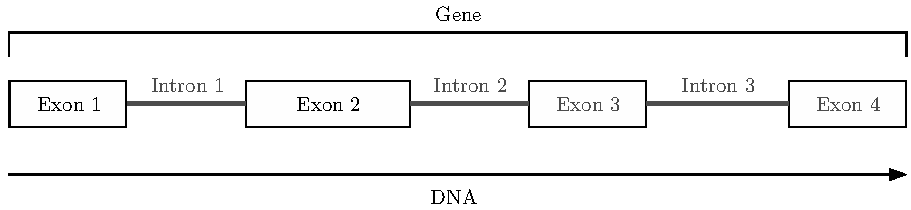
\includegraphics[width=1.0\textwidth]{intron_exon2}
    \caption[Overall structure of a gene]{Overall structure of a gene, with its
    different areas (simplified).}
    \label{fig:intron_exon}
  \end{center}
\end{figure}

The exons are useful in the gene expression process, being also known as coding
regions. Introns, on the other hand, are not used in the process. They are
present in an early stage mRNA molecule, the precursor mRNA, but are later
removed (or spliced) in the final molecule before the translation stage
\cite{leic:gene_expr}. Figure \ref{fig:splicing} illustrates the removal of
introns from the mRNA molecule, during the  splicing process.

\begin{figure}[!htb]
  \begin{center}
    \leavevmode
    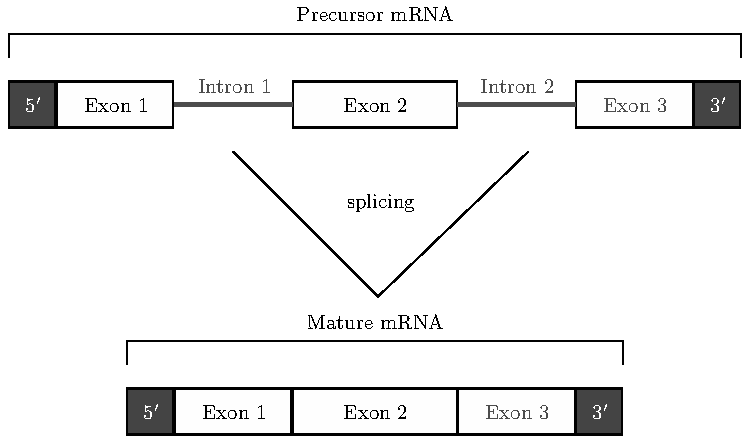
\includegraphics{splicing2}
    \caption[Removal of introns from precursor mRNA]{The removal (splicing) of
    introns from the precursor mRNA, during the transcription process.}
    \label{fig:splicing}
  \end{center}
\end{figure}

After the conclusion of the transcription process comes the translation process.
In this process, the synthesized mRNA is used to specify the sequence of amino
acids that constitute the particular protein being produced. The other types of
RNA molecules (rRNA and tRNA) are also used in this stage of the gene expression
process.

\subsection{RNA-Binding Proteins}

RNA-binding proteins, also referred to as RBP, regulate every aspect of the RNA
metabolism, including pre-mRNA splicing, mRNA transport, location, stability and
translation control \cite{Cooper2009777, Muller-McNicoll2013, Sonenberg2007721,
Sonenberg2009731}, as shown in Figure \ref{fig:rbp}.

\begin{figure}[!htb]
  \begin{center}
    \leavevmode
    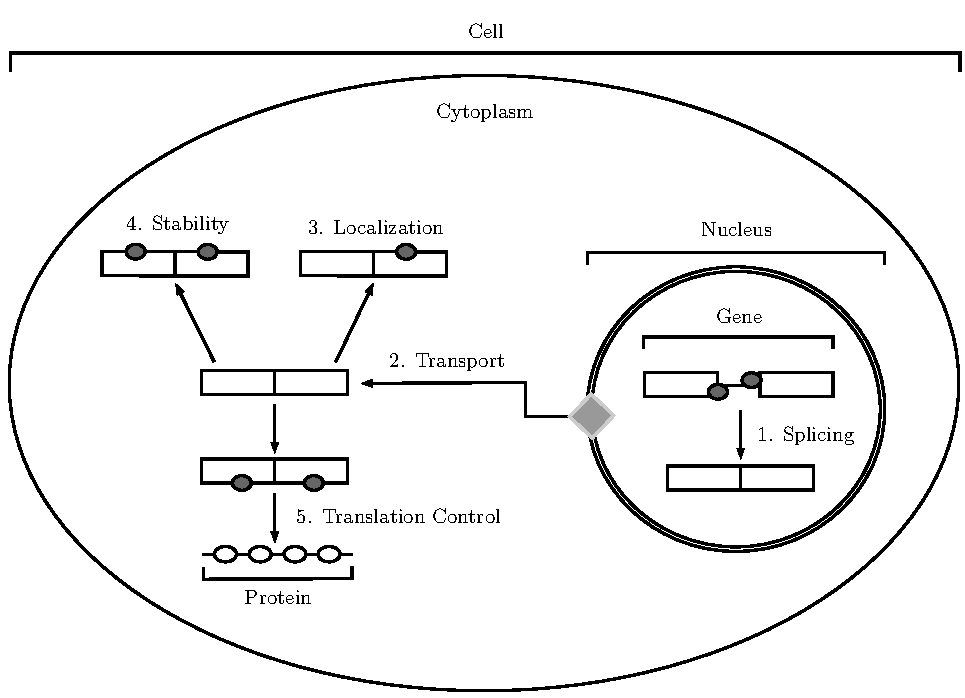
\includegraphics[width=\textwidth]{rbp}
    \caption[Role of RBPs in the RNA metabolism process]{
      Diagram of a typical cell showing the multiple roles of RBPs in post
      transcriptional processes \cite{janga2011construction}. The grey ellipses
      represent RBPs. The numbered text represents the different processes in
      which RBPs take part. Multiple RBPs can bind with a single RNA at one or
      more locations, creating an abundance of different combinations and
      possibilities in every step of the RNA metabolism.
    }
    \label{fig:rbp}
  \end{center}
\end{figure}

The binding of RBPs to RNA depends on different RNA-sequence specificities and
affinities. This aspect, coupled with the existence of hundreds of RBPs in an
organism, gives rise to a plethora of different combinations and outcomes to the
RNA metabolism.

RBPs regulate gene expression in health and disease, and mutations affecting the
function of RBPs may cause several diseases \cite{Cooper2009777}. Therefore,
understanding the binding patterns of RBPs during a particular biological
process is crucial to get insight into that process, both during health and
disease conditions.

\subsection{Sequencing}

Obtaining genetic information is done experimentally, by employing a sequencing
technique. For quite some time this process was carried out using the Sanger's
and other similar sequencing methods methods \cite{Reis-Filho2009}. Though
effective, such methods were notably slow and costly, with large projects like
the Human Genome Project (HGP) consuming roughly thirteen years and US\$ 3
billion. These limitations were so severe that, other than the realm of human
genetics, this kind of study was restricted to model organisms, such as the
fruit fly and mouse genomes \cite{Wolf2013}. The past few years have seen the
appearance and rise in popularity of the \ngs{} techniques. These techniques
differ from the more classical ones by producing larger amounts of information,
at lower cost. They are also typically more cost effective than previous
techniques and can be easily employed by single laboratories, which has greatly
contributed to their popularity.

The rise in popularity and availability of \ngs{} techniques, coupled with the
importance of RNA knowledge in understanding gene expression, led to the
appearance of RNA-Seq. RNA-Seq makes use of these newly available
deep-sequencing techniques to profile complete transcriptomes. This is, however,
a difficult task to accomplish. \ngs{} techniques produce shorter reads than
their older counterparts, being that \qt{\textit{(...) transcriptome assembly
from billions of RNA-Seq reads (...) poses a significant informatics challenge}}
\cite[p. 671]{Martin2011}.

Although this thesis does not deal with the problems of sequencing techniques, it
is important to indicate that the read data sets that were used resulted from
\ngs{} techniques, in particular RNA-Seq. As such, suitable tools for this
particular type of data were used.

\subsection{\Trans{} Assembly}

\Trans{} assembly is the process by which experimentally obtained RNA data reads
can be organized and merged together in a partial or complete \trans. As stated
above, the advent of next generation sequencing techniques, with their reduced
costs, greatly increased the availability of transcript sequencing data.

For years, microarrays were the standard tool available for examining features
of the transcriptome and global patterns of gene expression \cite{Wolf2013}.
However, microarrays are typically more oriented towards assembly against
existing reference data, hence limiting its application to species with well
known reference genomes. This is impractical, as \ngs{} techniques allow to
cheaply obtain genetic information of previously non-studied species. This is
one of the reasons that led to the inception of RNA-Seq. Contrary to
microarrays, RNA-Seq techniques are able to wield results that are suitable for
both reference guided assembly and \textit{de novo} assembly approaches
\cite{Wilhelm2009}. \textit{De novo} or exploratory assembly has captured the
interest of researchers in the past few years, leading to the appearance of
multiple RNA-Seq tools that are capable of making this type of assembly without
a reference genome \cite{nuno11:assemblathon}. Transcriptome assembly was not
performed during this thesis, as its main focus in terms of the RNA-Seq process
is read alignment and differential expression analysis.

\section{RNA-Seq Analysis}

\begin{Notes}
- Describe the same workflow as iRAP.\\
- Refer that we'll talk about specific tools below, and they all are Unix
command line tools.
\end{Notes}

\subsection{RNA-Seq Pipeline}

\begin{figure}[!htb]
  \begin{center}
    \leavevmode
    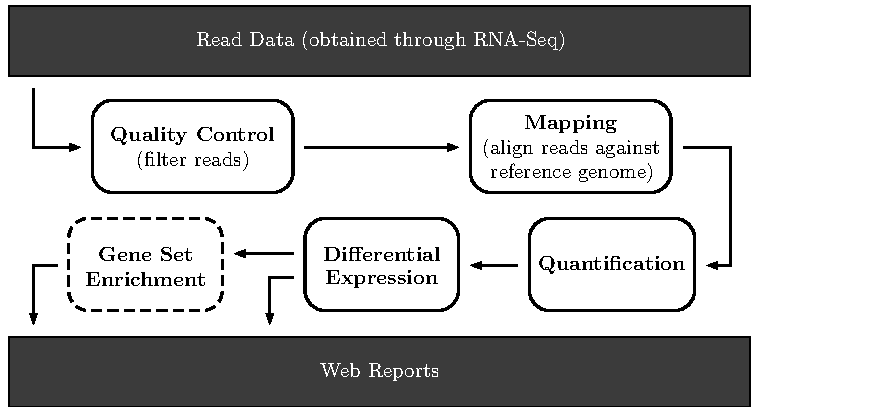
\includegraphics{irap}
    \caption[iRAP RNA-Seq data analysis pipeline]{
      iRAP RNA-Seq data analysis pipeline. Note that the gene enrichment step
      (in dashed line) is optional and was not used.
    }
    \label{fig:irap}
  \end{center}
\end{figure}

\subsection{\rnaseq{} Read Alignment and Analysis Tools}

Below we present some bioinformatic tools, used to support the multiple steps of
the \rnaseq{} read alignment and data analysis process. It is important to note that none of these
tools were used separately, but rather as parts of an analysis pipeline (also
described below).

\subsubsection*{Tuxedo Suite}

The Tuxedo suite is a free, open-source collection of applications that has been
widely adopted as analysis toolset for fast alignment of short reads. It is
composed by four separate tools, Bowtie, TopHat, Cufflinks and CummRbund,
briefly reviewed below. These tools are extensively used for \rnaseq{} analysis.
Although the applications are made for command line execution, there are several
workflow managers, like Galaxy\footnote{\url{http://galaxyproject.org/}}, that
easily integrates with the suite, providing a web interface for its use. Note
that not all components of the Tuxedo Suite were used.

\paragraph{Bowtie}

Bowtie is an ultrafast, memory-efficient short read aligner
\cite{langmead2009ultrafast}. Bowtie is typically used to build a reference
index for the genome of the organism being studied, for posterior use by other
tools, like TopHat. It can also output alignments in the standard SAM format,
allowing Bowtie to interoperate with tools like SAM Tools. However, it should
not be used as a general purpose alignment tool, as it was created and is more
effective when aligning short read sequences against large reference genomes.

\paragraph{TopHat}

TopHat is a fast splice junction mapper for \rnaseq{} reads
\cite{Trapnell01052009}. It uses Bowtie as the underlying alignment tool, using
its results and a FASTA formated reference genome to identify splice junctions
between exons.

\paragraph{Cufflinks}

Cufflinks assembles transcripts, estimates their abundances, and tests for
differential expression and regulation in \rnaseq{} samples
\cite{trapnell2010transcript}. It uses the SAM or BAM formatted files as input,
typically the ones produced by TopHat, outputting GTF files as a result.

\paragraph{CummeRbund}

Lastly, CummeRbund\footnote{\url{http://compbio.mit.edu/cummeRbund/}} is an R
package (see Section \ref{sec:mintools}) designed to help the visualization and
analysis of Cufflinks' \rnaseq{} output. As such, it is not directly involved in
the trascriptome alignment process. It takes the various output files from
Cufflinks and uses them to build a SQLite database describing appropriate
relationships between genes, transcripts, etc. This database is later used to
convert that data to R objects which allows them to be used the included
plotting functions, as well as in other commonly used data visualizations.

\subsubsection*{HTSeq}

HTSeq is a programming framework used for processing data resulting from next
generation sequencing methods \cite{htseq}, developed in Python. While many
tools can efficiently align reads, sometimes data needs to be manipulated before
being passed to those tools. This data can either be badly formated (or
\qt{dirty}) or simply in a format different from the one that is needed. The
latter is a particularly common problem when trying to pass the results of one
tool to the one that succeeds it in the pipeline. HTSeq is useful to easily
create scripts that accomplish this task, acting as a \qt{glue} between tools.

HTSeq provides parsers for many popular formats for representing genetic
information (see Section \ref{sec:formats}). In addition, it ships with two
standalone scripts, HTSeq-QA and HTSeq-Count. HTSeq-QA is used to provide an
initial assessment of the quality of sequencing runs, producing plots with that
information. HTSeq-Count takes a SAM/BAM file and GTF/GFF file containing gene
models. It then counts, for each gene, how many aligned reads overlap that
gene's exons.

\subsection{Differential Expression Analysis Tools}

Below we describe the tools that were used for differential expression analysis.
These tools are integrated in the iRAP pipeline, and make are used in its fourth
stage.

\subsubsection*{DESeq}

DESeq in an R package (see Section \ref{sec:mintools}), included in the
Bioconductor super package \cite{20979621}. DESeq takes count data generated
from RNA-Seq analysis assays. As count data is discrete and skewed, it is not
well approximated by a normal distribution. DESeq solves this problem by
applying a test based on the negative binomial distribution, which can reflect
these properties. This method has a much higher power to detect differential
expression.

\subsubsection*{edgeR}

edgeR in an R package (see Section \ref{sec:mintools}), included in the
Bioconductor super package \cite{robinson2010edger}. It provides methods for the
statistical analysis of count data from comparative experiments on next
generation sequencing platforms, among which is RNA-Seq, the most common source
of data used with edgeR. It has many characteristics in common with the
previously mentioned DESeq, as it also uses negative binomial models (among
others) to distinguish biological from technical variation. Later we describe
how both tools can be used together to produce better results.

\subsection{File Manipulation and Pre-processing Tools}

Sometimes data is badly formated or otherwise in a format that is not compatible
with a specific tool. This is particularly frequent when passing data between
two different tools in a pipeline. As such, we need some intermediate tools that
are able to easily manipulate and transform data, making it useful again. Below
we present some tools that can be used to accomplish this task.

\subsubsection*{SAM Tools}

SAM Tools\footnote{\url{http://samtools.sourceforge.net/}} is a library
package designed for parsing and manipulating alignment files in the SAM/BAM
format \cite{Li2009} (see Section \ref{sec:formats}). SAM Tools has two separate
implementations, one in C and the other in Java, with slightly different
functionality. Beyond manipulation of SAM and BAM files, this package is able to
convert between other read alignment formats, sort and merge alignments and show
them in a text-based viewer.

\subsubsection*{BLAST}

BLAST\footnote{\url{http://blast.ncbi.nlm.nih.gov/Blast.cgi}} is a tool,
implemented in C++, that is used to find regions of local similarity between
biological sequences. It uses FASTA sequences (see Section \ref{sec:formats}) as
search input and outputs the results reports in XML, HTML or plain text. There
are several different BLAST programs available at the moment, that can be used
depending on our objective and type of data. BLAST is particularly useful to
search biologic sequence databases, but can be used for other purposes, like
identifying an unknown species or comparing common genes in two related
species.

\subsubsection*{FASTX}

\subsubsection*{FastQC}

\subsection{Relevant Standard File Formats}\label{sec:formats}

As expected, the great diversity of RNA-Seq tools brings with it a wealth of
file formats. Some of these formats are developed from the ground up to satisfy
a specific need, while others are mere contextual adaptations or specializations
of already established formats. Below we will present a few of the most popular
and widely spread file formats, talking about their basic structure, the types
of data they represent and their applications.

\subsubsection*{FASTA}

FASTA is the standard line and character sequence format used by NCBI
\cite{ncbi:fasta}, using this last organization's character code conventions. It
is a simple format, that can be used to easily store data represented by
character sequences, like nucleotide (\dna, \rna) or amino acid (protein)
sequences. This file format is widely use to store sequencing reads, \dna/\rna{}
sequences and other character sequences in database systems. Its simplicity
makes it extremely easy to manipulate and parse, presenting also an attractive
solution for data transfer between different tools.

\subsubsection*{FASTQ}

FASTQ is used to store store character sequences, typically nucleotide sequences
\cite{Cock2010}. It is quite similar to the standard FASTA format, in respect to
the manner in which character sequences are represented. However, for every
sequence, there is a second sequence of equal length, representing the quality
scores of the original sequence. These quality scores are also represented as
single characters, taking values between and including ASCII-33 to ASCII-126.
It is typically used in the same situations as the FASTA format, when quality
scores are available/relevant.

\subsubsection*{SAM and BAM}

The SAM format is a text format for storing sequence alignment data
\cite{genome:sam}. It is widely used to store mapping information between
sequencing reads and a given reference genome. This sort of information is
typically the product of sequencing alignment tools, that consume sequencing
reads from FASTQ files and align them with a reference genome.

The BAM format contains exactly the same information as the SAM format and the
same rules apply for both formats. The difference between both formats lies in
their encoding. While SAM is a text based format, BAM is a binary format. This
means that BAM sacrifices human readability for increased machine processing
performance, as it is more efficient to work with compressed and indexed binary
data.

\subsubsection*{VCF}

VCF is a text file format used to store gene sequence variants \cite{smith13}.
In the past few years, as larger and larger genome sequencing projects became
more common (like the 1000 Genomes Project\footnote{The 1000 Genomes Project,
started back in 2008, is an international effort to establish the most
comprehensive catalogue to date of human genetic variations.}), storing such
large amounts of information became a serious concern. To address these concerns
the VCF format was created. Instead of storing the complete genome, VCF stores
only the variations (and their respective positions) of newly sequenced genomes
relatively to a known reference genome, typically in a compressed text file. As
such, it is a format often used when building genome databases.

\subsubsection*{GFF and GTF}

GFF is a text based file format to store gene features \cite{sanger11}. Many
genome assembly tools execute this process in two separate steps: feature
detection for identification of specific regions (exons, introns, etc.) and
genome assembly, using those features as reference. However, often times it is
beneficial to decouple these two steps, using different and more efficient tools
for each. As such, the GFF format emerged as a protocol for feature information
transfer between tools.

The GTF format is similar to the GFF format, in which it is based. It is also
used in similar situations. However, GTF builds on top of GFF, defining
additional conventions, specific to the domain of genetic information. Despite
their initial relation, both formats continue to be developed individually.

\section{Data Mining}\label{sec:mlearning}

\begin{Notes}
- Still relevant, don't change.\\
- Important part is now clustering, not classification.
\end{Notes}

Data mining is the process of \qt{\textit{extracting or \qt{mining} knowledge
from large amounts of data}} \cite[p. 5]{han2006data}. As such, it consists of a
set of techniques that can be used to find interesting patterns in large data
sets, that translate in newfound knowledge. Data mining borrows techniques from
multiple fields, such as artificial intelligence, machine learning, statistics,
and database systems \cite{Chakrabarti2012}. Its ultimate goal is to combine all
those techniques and transform large and (apparently) meaningless sets of data
into understandable and useful information. Thus, data mining was motivated by
the perspective of harnessing the abundance of data, that characterizes today's
information systems, to produce meaningful knowledge.

Because of their large quantities of input data, data mining tasks are usually
totally, or at least partially, automated. As such, there are several algorithms
for these tasks and tools that implements such algorithms, as presented in
Section \ref{sec:minalgo} and Section \ref{sec:mintools}, respectively.

We can divide data mining into main types: descriptive data mining and
predictive data mining \cite{Fayyad1996}. Descriptive data mining is focused on
finding the underlying structure of a given set of data. Instead of predicting
future values, it concerns the intrinsic structure, relations and
interconnectedness of the data being analyzed, presenting its interesting
characteristics without having any predefined target. On the other hand,
predictive data mining is used to predict explicit values, based on patterns
determined from the dataset. With predictive data mining we try to build models
using known data and use those models as a base to predict future behavior.

As we're seeing, data mining does not represent a single type problem. In fact
there are several different types of problems that can be addressed by data
mining techniques. Each of these problems may require a different data mining
method. A brief review of the most common methods is given below.

\begin{description}

  \item[Classification]
  is a method that tries to generalize the already known structure of a
  dataset, so that it applies to new datasets. In other words, with
  classification we try to learn a function that is capable of mapping our data
  into predefined classes.

  \item[Regression]
  tries to learn a function that models relationships between variables in the
  dataset. That function can latter be used to find real value predictions of
  future behavior of the same or similar datasets.

  \item[Clustering]
  consists in identifying a finite set of categories or clusters of similar
  values, to describe the dataset. As such, it is used without prior knowledge
  about data structure.

  \item[Summarization]
  provides a more compact representation of a subset of data, in a way that the
  summarized data retains the central points of the original data. This can be
  accomplished in several different ways, like using report generation or
  multivariate visualization techniques.

  \item[Dependency modeling]
  finds a model which describes relationships between variables, revealing their
  dependencies.

  \item[Change and deviation detection]
  tries to discover the most significant changes in the data, when compared with
  previously measured data. This method is useful to find interesting data
  variations or data errors.

\end{description}

\subsection{Data Mining Algorithms}\label{sec:minalgo}

\begin{Notes}
- Focus is now on clustering algorithms.
- See Wikipedia's page on "clustering" for a good reference on algorithm types.\\
\end{Notes}

In this project we will be concerned with the classification side of data
mining. Below, we will review some algorithms that can be used in
classification problems.

%\subsubsection*{Decision Trees}

%\textit{\qt{A decision tree is a flowchart-like tree structure, where each
%internal node (nonleaf node) denotes a test on an attribute, each branch
%represents an outcome of the test, and each leaf node (or terminal node) holds a
%class label}} \cite[p. 291]{han2006data}, as seen in Figure \ref{fig:tree}.
%Decision tree learning algorithms use a decision tree as a predictive model,
%that maps observed data about an individual to conclusions about the expected
%value for that individual. From a classification problem standpoint, this means
%means creating a decision tree structure that is able to predict the class of an
%individual based on its attributes.

%\begin{figure}[htb]
  %\centering

  %% Node levels and identation.
  %\tikzstyle{level 1}=[level distance=1.5cm, sibling distance=4.25cm]
  %\tikzstyle{level 2}=[level distance=1.5cm, sibling distance=2.25cm]
  %\tikzstyle{level 3}=[level distance=1.5cm, sibling distance=4.25cm]
  %\tikzstyle{level 4}=[level distance=1.5cm, sibling distance=2.25cm]

  %% Node style.
  %\tikzset{decision/.style={
    %draw=black!80, solid, fill=white!10, rectangle,
    %anchor=north,
    %inner sep=2mm, outer sep=0, text centered, growth parent anchor=south}
  %}
  %\tikzset{prediction/.style={
    %draw=black!80, solid, fill=white!30, ellipse,
    %anchor=north,
    %inner sep=2mm, outer sep=0, text centered, growth parent anchor=south,
    %minimum height=1cm,minimum width=1.3cm}
  %}

  %% Tree.
  %\begin{tikzpicture}
    %\node [decision] {\textit{age?}} [solid, -latex, thick, -]
      %child {
        %node [decision] {\textit{student?}} [solid, -latex, thick, -]
        %child {
          %node [prediction] {no} [solid, -latex, thick, -]
          %edge from parent
          %node[left] {no}
        %}
        %child {
          %node [prediction] {yes} [solid, -latex, thick, -]
          %edge from parent
          %node[right] {yes}
        %}
        %edge from parent
        %node[above left] {youth}
      %}
      %child {
        %node [prediction] {yes} [solid, -latex, thick, -]
        %edge from parent
        %node[below,fill=white,inner sep=1pt] {middle\_aged}
      %}
      %child {
        %node [decision] {\textit{credit\_rating?}} [solid, -latex, thick, -]
        %child {
          %node [prediction] {no} [solid, -latex, thick, -]
          %edge from parent
          %node[left] {no}
        %}
        %child {
          %node [prediction] {yes} [solid, -latex, thick, -]
          %edge from parent
          %node[right] {yes}
        %}
        %edge from parent
        %node[above right] {senior}
      %}
    %;
  %\end{tikzpicture}
  %\caption[Example of a decision tree]
  %{Example of a decision tree for the concept \textit{buys\_computer},
  %indicating whether a customer is likely to purchase a computer. Each internal
  %(nonleaf) node represents a test on an attribute. Each leaf node represents a
  %class (either \textit{buys\_computer = yes} or \textit{buys\_computer = no})
  %\cite[p. 291]{han2006data}.}
  %\label{fig:tree}
%\end{figure}

%Decision tree classifiers are among the most popular used nowadays. They are
%able to handle high dimensional data and their learning and classification steps
%are simple and fast. Other than that, the construction of decision tree
%classifiers does not not require domain knowledge or parameter setting. These
%classifiers usually have a good level of accuracy, though it may vary with the
%type of data available.

%That are several algorithms that use the decision tree principle, most notably
%\textit{ID3}, \textit{C4.5} and \textit{CART}. As the problem of learning an
%optimal decision tree is NP-complete, most algorithms for decision tree
%construction are based in some sort of heuristics (the aforementioned algorithms
%adopt a greedy approach).

%\subsubsection*{Random Forest}

%Random forest \cite{breiman2001random} is an ensemble approach for
%classification and regression problems. Ensembles use a divide-and-conquer
%approach to classification problems, in order to increase performance. The base
%principle behind ensembles is simple: a group of \qt{weak} learners can come
%together to become a \qt{strong} learner, where their individual shortcomings
%are amortized by their combined results. As such, random forest algorithms use
%several individual decision trees, in order to mitigate the problems with
%variance and bias in single decision trees.

%Each individual tree in the forest in trained used a random subset of the
%original dataset, where the subsets distribution is the same across the forest.
%Then, at each node we choose the predictor variable that provides the best split
%(as per an objective function) and use it to do a binary split at that node.
%This continues until all the trees are grown to the largest extent possible, as
%no pruning is made.

%Random forest is a fairly fast method and is able to deal with unbalanced and
%missing data. It as few parameters to tune and can be easily and effectively
%used with default parameters. As a limitation, when used for regression random
%forests cannot predict beyond the range in the training data, and that they may
%overfit datasets that are particularly noisy.

%\subsubsection*{Support Vector Machines}

%Support vector machines are a set of related supervised learning methods used
%for pattern recognition, that can be applied to classification and regression
%problems \cite{Cortes1995}. SVMs typically fall under a simple premise, the
%spacial division of classes. As seen in Figure \ref{fig:svm}, we can define an
%infinite number of possible separating hyperplanes or \qt{decision boundaries}
%(in this case straight lines). The objective of an SVM is to find the optimal
%hyperplane or set of hyperplanes to separate the classes. To classify a new set
%of data each value is represented in the space and classified according to the
%side of the hyperplane in which it falls.

%\begin{figure}[!htb]
  %\begin{center}
    %\leavevmode
    %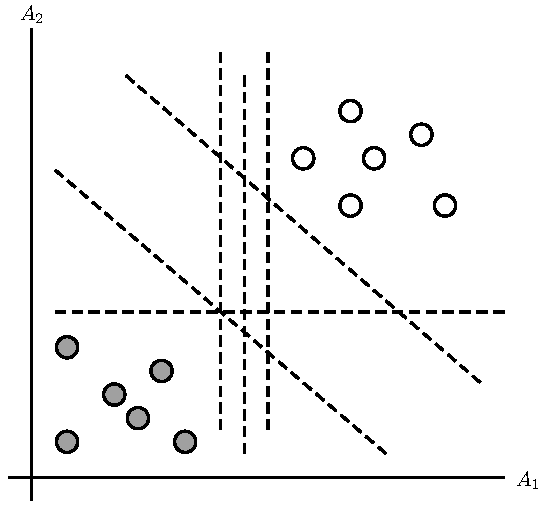
\includegraphics[width=0.6\textwidth]{svm2}
    %\caption[Example of linearly separable training data]
    %{Example of linearly separable training data in a two dimensional
    %space. There are an infinite number of (possible) separating hyperplanes or
    %\qt{decision boundaries} \cite[p. 338]{han2006data}.}
    %\label{fig:svm}
  %\end{center}
%\end{figure}

%SVMs are widely used nowadays, and have been successfully applied in areas such
%handwritten digit recognition, object recognition, and speaker identification,
%as well as benchmark time-series prediction tests \cite{han2006data}. They are
%typically regarded. They are highly accurate, due in part to their ability to
%model complex nonlinear decision boundaries.

%However, even the fastest SVMs can be extremely slow in both the training and
%testing steps. It is also directly limited to two-class tasks, requiring the use
%of other algorithms to reduce multi-class tasks to binary ones.

%\subsubsection*{K-NN}

%K-NN is a non-parametric method for classification and regression problems.
%First described in the early 1950s \cite{han2006data}, it is one of the simplest
%machine learning algorithms and is widely used in the area of pattern
%recognition.

%Nearest neighbor classifiers are based on the premise of learning by analogy, in
%other words, by comparing a given test tuple with similar training tuples. This
%classification of tuples as \qt{similar} is typically based on simple rules,
%like the \textit{Euclidean distance} between tuples.

%In k-NN, each training tuple is described by $n$ attributes and is represented
%as a point in an $n$-dimensional space. For classification problems, the test
%tuple is represented in this space, along with the training tuples. The unknown
%tuple is then assigned to the most common class among its $k$ nearest neighbors.

%K-NN as several advantages when compared to other classification algorithms. For
%one it has a very simple implementation. it is also very robust in terms of
%search space (the classes don't have to be linearly separable) and has few
%parameters, making it easy to tune. On the other side, it is an expensive method
%in terms of testing, as we need to calculate the distance between a testing
%tuple and every other known tuple. Furthermore, it is sensitive to noisy or
%irrelevant attributes and unbalanced datasets.

\subsubsection*{Inductive Logic Programming}

\begin{Notes}
- Still seems relevant, later refer that it wasn't possible to conduct ILP
clustering due to lack of time/problems with tools.\\
\end{Notes}

ILP is a subfield of machine learning that uses first order logic to represent
both data and models \cite{Lavrac1998}. ILP induces hypotheses (models) from
examples and background knowledge. Examples are of two types: instances of the
concept to be \qt{learned} and non-instances of the concept. Background
knowledge is a set of predicates encoding all information that the experts find
useful to construct the models. ILP might be used to tackle several machine
learning and data mining problems, like classification, regression and
clustering.

The first and most important motivation for ILP systems is that they overcome
the representation limitations of attribute-value learning systems, such as the
previously mentioned data mining algorithms. Attribute-value systems base their
representations of data in table based representations. Although effective in
many situations, these representation is not very expressive and might not even
be feasible for certain problems \cite{Bratko:1995:AIL:219717.219771}. The
second motivation for ILP is that by using a logical representation, the
hypotheses are understandable and interpretable by humans, being therefore
useful to explain the phenomenons that produce the data. This representation
also means that background knowledge can be represented and employed in the
induction process, in contrast to attribute-value models, where this information
is difficult to represent.

Despite these advantages, ILP cannot be applied indiscriminately to any
classification or regression problem. ILP systems are typically very heavy when
it comes to computational resource consumption and run for long periods of time
\cite{fonseca2003implementation}.

\subsection{Model Evaluation Procedures and Measures}\label{sec:mineval}

\begin{Notes}
- No longer relevant.\\
- Explain internal and external evaluation.\\
- Explain that due to the novelty of our analysis we will merely focus on
internal analysis.\\
- Describe some internal analysis measures (don't forget silhouettes).\\
\end{Notes}

%Creating a data model using a suitable classification algorithms is not the last
%step in the data mining process. At this point our model works well with the
%original training data, but we need to verify its power to generalize to other
%sets of data. Without this evaluation process, our models may be susceptible to
%problems like overfitting, in which the model wrongly describes a random error
%or data noise as a significant pattern \cite{han2006data}. As such, we need
%methods that allow us to test our models before deployment, as well as standard
%measures, to determine their quality.

%\subsubsection*{Evaluation Procedures}

%As stated, evaluation procedures are essential to verify the generalization
%capabilities of a given model. These procedures typically consist of dividing
%the test dataset in two or more subsets, using some of them for training and the
%others for testing. We will present a brief overview of some of these procedures
%below.

%\paragraph{Hold-Out}

%The \textit{hold-out} method reserves a part of the dataset for training
%purposes and uses the remaining data for testing \cite{witten2011data}.
%Typically we separate one third of the original dataset for testing, using the
%other two thirds for training.

%However, this arbitrary division of the dataset might be problematic if the
%subsets aren't representative of the population. For example, if the test subset
%is missing a class our results might be erratic. One way to attenuate this
%problem is to use stratification. Using stratification of the dataset we ensure
%that both subsets are representative, with approximately equal proportions for
%each class. We can lessen error rates even further and make the
%\textit{hold-out} estimate more reliable using the \textit{repeated hold-out}
%method. This is an iterative method, where in each iteration a subset is
%randomly selected to use as training (possibly using set stratification), using
%the remaining subset for testing. After all the iterations, the error rates of
%each one are averaged to yield an overall error rate.

%\paragraph{Cross-Validation}

%\textit{Repeated hold-out} methods pose a problem: the different test subsets
%will eventually overlap. This may cause that some examples never appear in the
%training subsets. The overlapping problem can be solved using the
%\textit{cross-validation} procedure, also called \textit{k-fold
%cross-validation}. This method consists in splitting the original dataset into
%\textit{k} subsets, using each subset in turn for testing and the remainder for
%training.

%The standard method for evaluation is \textit{10-fold cross validation}, where
%the dataset is divided into ten subsets. The subsets are typically stratified to
%reduce result variance. In each iteration one of the ten folds is picked as test
%and the other nine are used for training. Sometimes, to further reduce variance,
%\textit{repeated stratified cross-validation} is used, repeating normal
%\textit{10-fold cross-validation} ten times, then averaging the results.

%\paragraph{Leave-One-Out}

%\textit{Leave-one-out} method is a form of \textit{cross-validation}, taken to
%extreme lengths. In this particular method, the original dataset is divided into
%\textit{n} folds, where \textit{n} is the number is the number of individual
%training instances. It has some benefits, like allowing for a better use of the
%dataset and involving no random set sampling. However, the sheer number of folds
%and tests makes it a very computationally expensive method. Another disadvantage
%is that no stratification is possible, as there is always only one instance in
%the test subset.

%\subsubsection*{Common Measures}

%Applying evaluation procedures is not sufficient by itself. In order to appraise
%the quality of our models, we need to use standard quality measures, that give
%meaning to the obtained results. Below we will review some common measures, used
%in the context of classification problems.

%\paragraph{Precision}

%Precision determines the fraction of positive cases that are correctly
%identified as such. Low precision values mean that the model identifies many
%cases as positive when they are in reality false positives. Precision is
%calculated as shown in Equation \ref{eq:precision}.

%\begin{equation}
  %Precision=\frac{\tp}{\tp + \fp}
  %\label{eq:precision}
%\end{equation}

%\paragraph{Recall}

%Recall represents the portion of actual positive results in the dataset that
%were identified as such. From a statistical standpoint, it can be viewed as the
%average probability of find all the positive cases in the dataset. The value is
%computed using Equation \ref{eq:recall}.

%\begin{equation}
  %Recall=\frac{\tp}{\tp + \fn}
  %\label{eq:recall}
%\end{equation}

%\paragraph{Accuracy}

%Accuracy represents the percentage of predictions that are in fact correct. This
%measure relates to the ability of our model to correctly predict the class of
%new data. It can be calculated with Equation \ref{eq:accuracy}. For a given
%problem, better accuracy might not always mean that a model is better than
%another. As such, other measures like precision and recall are also taken into
%account.

%\begin{equation}
  %Accuracy=\frac{\tp + \tn}{\tp + \fp + \tn + \fn}
  %\label{eq:accuracy}
%\end{equation}

%\paragraph{F-Measure}

%F-measure is the harmonic mean of precision and recall. The reason behind the
%usage of an harmonic mean instead of an arithmetic mean is that the first is
%more intuitive, when computing a mean of ratios \cite{Sasaki2007}. F-measure is
%calculated as shown in Equation \ref{eq:fmeasure}. It is particularly useful to
%differentiate between cases where one of the variables (precision or recall) has
%a very high value and the other has a very low value. For example, if in a
%particular situation we have a precision of $1.0$ and a recall of $0.2$, the
%arithmetic mean would be $0.6$. However, a system with a recall as low as $0.2$
%might not be very useful. On the other hand, in the same situation the harmonic
%mean would be $0.333(3)$, giving a much more realistic measure of the quality of
%the model.

%\begin{equation}
  %\textit{F-measure}=2 \cdot \frac{\mathit{Precision} \cdot
  %\mathit{Recall}}{\mathit{Precision}+\mathit{Recall}} \label{eq:fmeasure}
%\end{equation}

%\paragraph{AUC}

%Sometimes in order to evaluate the quality of a certain model we might plot a
%ROC (or \textit{receiver operating characteristic}) curve. ROC curves depict the
%performance of a classifier without regard to class distribution or error
%costs. The curve is build by plotting false positive rates in the $x$ axis and
%true positive rates (recalls) in the $y$ axis (Figure \ref{fig:roccurve}).

%\begin{figure}[ht]
  %\begin{center}
    %\begin{tikzpicture}
      %\begin{axis}[
        %domain=0:1,
        %legend pos=south east,
        %xlabel=False Positive Rate,
        %ylabel=True Positive Rate]
        %\addplot[mark=none, samples=10, red] function {x};
        %\addplot[smooth, color=blue, mark=none]
          %plot coordinates {
              %(0.0,0.0)
              %(0.1,0.4)
              %(0.2,0.7)
              %(0.3,0.8)
              %(0.4,0.85)
              %(0.5,0.88)
              %(0.6,0.91)
              %(0.7,0.94)
              %(0.8,0.97)
              %(0.9,0.99)
              %(1.0,1.0)
          %};
        %\legend{Random model,Created model}
      %\end{axis}
    %\end{tikzpicture}
    %\caption[Example of ROC curve]{Example of ROC curve.}
    %\label{fig:roccurve}
  %\end{center}
%\end{figure}

%However, the curve can be hard to interpret at times. In this situation we can
%use the AUC measure (or \textit{area under the curve}), in order to condensate
%the curve's information in a single value. The AUC of a random classification
%system is $0.5$. This means that any model that as an AUC of $0.5$ is not able
%to distinguish between two groups. As the AUC increases, the model's quality
%also increases and at a value of AUC equal to $1.0$ the model is able to
%perfectly separate both groups.

\subsection{Data Mining Tools}\label{sec:mintools}

Except in rare cases of very specific problems, it typically makes no sense for
someone to implement any data mining algorithm that they might need. In fact,
today we have lots of data mining tools (many of which are free), that already
implement many of those algorithms. These tools are usually customizable, making
it easy to adapt them to most problems. Below we'll briefly review some of the
most popular data mining tools, that apply to the specific needs of this thesis.

\subsubsection*{RapidMiner}

\begin{Notes}
- Still relevant.\\
- Refer that RapidMiner and Weka were only used for testing purposes, and are
note part of the final solutions.\\
- Refer other relevant R packages.\\
\end{Notes}

RapidMiner\footnote{\url{http://www.rapidminer.com/}} is a complete solution for
data mining problems. it is available as a standalone GUI based application, as
seen in Figure \ref{fig:rapidminer}. It is a commercial application, although
its core and earlier versions are distributed under an open source license and
it offers a free version, beyond its multiple paid versions. Being one of the
most popular data mining tools used today, its applications span several
domains, including education, training, industrial and personal applications,
among others. Its functionality can also be easily extended through the use of
plugins\footnote{Plugin is a software module that adds new functionality to an
existing software application. Plugins are typically dependent on the platform
they extend and can't be used as standalone tools.}, reflecting in an increased
value for this tool. One such example in the area of bioinformatics is the
integration plugin between RapidMiner and the
Taverna\footnote{\url{http://www.taverna.org.uk/}} open source workflow
management system \cite{Jupp2011}.

\begin{figure}[!htb]
  \begin{center}
    \leavevmode
    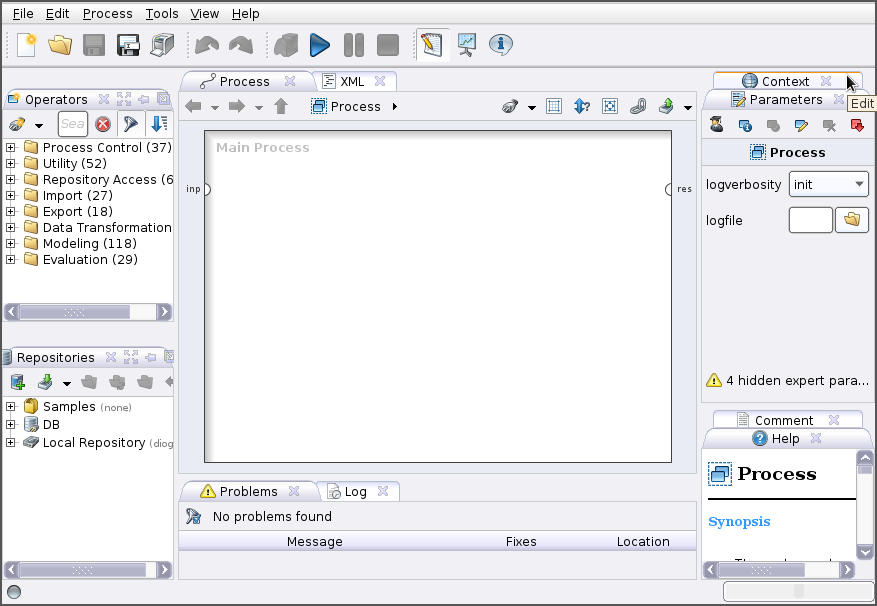
\includegraphics[width=1.0\textwidth]{rapidminer}
    \caption[RapidMiner user interface]{RapidMiner user interface.}
    \label{fig:rapidminer}
  \end{center}
\end{figure}

\subsubsection*{Weka}

Weka\footnote{\url{http://www.cs.waikato.ac.nz/ml/weka/}} is an open source tool that
collects several machine learning algorithms and allows its user to easily apply
those algorithms to data mining tasks \cite{Hall}. Created at the University of
Waikato, New Zeland in 1997 (the current version was completely rewritten in
1997, despite the first iteration of the tool being developed as early as 1993),
it is still in active development to date. Weka supports several common data
mining tasks, like data preprocessing, classification, clustering, regression
and data visualization. it is core libraries are written in Java and allow for an
easy integration of its data mining algorithms in pre existing code and
applications. Other than that, Weka can be used directly through a command
line/terminal or through one of its multiple GUIs (Figure \ref{fig:weka}). Its
simple API and well structure architecture allow it to be easily extended by
users, should they need new functionalities.

\begin{figure}[!htb]
  \begin{center}
    \leavevmode
    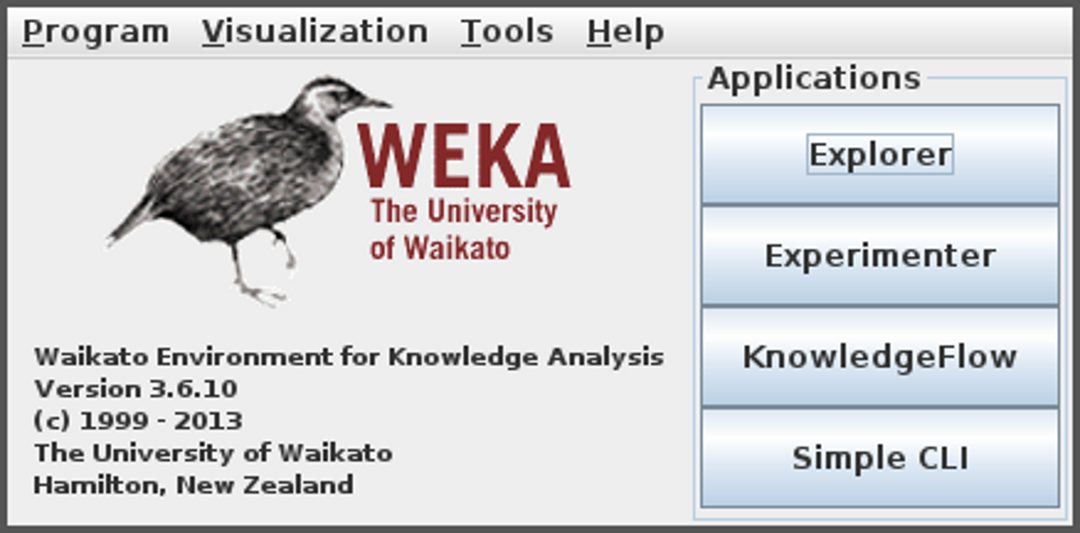
\includegraphics[width=0.7\textwidth]{weka}
    \caption[Weka interface selection]{Weka interface selection.}
    \label{fig:weka}
  \end{center}
\end{figure}

\subsubsection*{R Language}

R\footnote{\url{http://www.r-project.org/}} is a free programming language and
software environment for statistical computing and graphics generation.
Originally developed by Ross Ihaka and Robert Gentleman at the University of
Auckland, New Zealand in 1993 \cite{Ihaka1998}, it is still under active
development. R is typically used by statisticians and data miners, either for
direct data analysis or for developing new statistical software \cite{Fox2005}.

R is an implementation of the S programming language\footnote{S is an object
oriented statistical programming language, appearing in 1976 at Bell
Laboratories.}, borrowing some characteristics from the Scheme programming
language. it is core is written in a combination of C, Fortran and R itself. It
is possible directly manipulate R objects in languages like C, C++ and Java. R
can be used directly through the command line or through several third party
graphical user interfaces like
Deducer\footnote{\url{http://www.deducer.org/pmwiki/index.php}}. There are also
R wrappers for several scripting languages.

R provides several different statistical and graphical techniques, including
linear and nonlinear modeling, classical statistical tests, time-series
analysis, classification, clustering, among others. It can also be used to
produce publication-quality static graphics. Tools like Sweave
\cite{lmucs-papers:Leisch:2002} allow users to embed R code in \LaTeX{}
documents, for complete data analysis.

\paragraph{Bioconductor Package}

Bioconductor is a free and open source set of tools for genomic data analysis,
in the context of molecular biology \cite{lmucs-papers:Leisch:2002}. It is
primarily based on R. It is under active development, with two stable releases
each year. Counting with more than seven hundred different packages, it is the
most comprehensive set of genomic data analysis tools available for the R
programming language. It also provides a set of tools to read and manipulate
several of the most common file formats used in molecular biology oriented
applications, including FASTA, FASTQ, BAM and GFF.

\section{Chapter Conclusions}

\begin{Notes}
- Remove the uncertainty part, talk about what was done.\\
\end{Notes}

In this chapter we gave a brief introduction of the molecular biology concepts
that serve as base of the thesis. We also reviewed the concepts on RNA-Seq and
data mining and presented short analyses of concrete tools that will likely be
used during the project.

At this moment we do not possess all the necessary information about the dataset
that will be used in the data mining phase of the project. We are unable, at the
present, to determine the nature of our data, which means that we cannot predict
whether it could be modeled by classification algorithms. As such, we presented
ILP as an alternative approach for this situation. In case ILP techniques become
in fact necessary, further work will include a more profound and complete
revision.

%\chapter{Visualização de Sinópticos SVG}\label{chap:chap3}

\section*{}

Este capítulo deve começar por fazer uma apresentação detalhada do
problema a resolver\footnote{Na introdução a apresentação do
  problema foi breve.} podendo mesmo, caso se justifique,
constituir-se um capítulo com essa finalidade.

Deve depois dedicar-se à apresentação da solução sem detalhes de
implementação. 
Dependendo do trabalho, pode ser uma descrição mais teórica, mais
``arquitetural'', etc.

\section{Secção Exemplo}

Neste capítulo apresentam-se exemplos de formatação de figuras e
tabelas, equações e referências cruzadas.

Apresenta-se de seguida um exemplo de equação, completamente fora do contexto:
\begin{eqnarray}
CIF_1: \hspace*{5mm}F_0^j(a) &=& \frac{1}{2\pi \iota} \oint_{\gamma} \frac{F_0^j(z)}{z - a} dz\\
CIF_2: \hspace*{5mm}F_1^j(a) &=& \frac{1}{2\pi \iota} \oint_{\gamma} \frac{F_0^j(x)}{x - a} dx \label{eq:cif}
\end{eqnarray}

Na Equação~\ref{eq:cif} lorem ipsum dolor sit amet, consectetuer
adipiscing elit. Suspendisse tincidunt viverra elit. Donec tempus
vulputate mauris. Donec arcu. Vestibulum condimentum porta
justo. Curabitur ornare tincidunt lacus. Curabitur ac massa vel ante
tincidunt placerat. Cras vehicula semper elit. Curabitur gravida, est
a elementum suscipit, est eros ullamcorper quam, sed cursus velit
velit tempor neque. Duis tempor condimentum ante.

Phasellus imperdiet, orci vel pretium sollicitudin, magna nunc
ullamcorper augue, non venenatis dui nunc quis massa. Pellentesque
dolor elit, dapibus venenatis, viverra ultricies, accumsan cursus,
orci. Aliquam erat volutpat. Mauris ornare tristique leo. Maecenas
eros. Curabitur velit nunc, tincidunt vitae, dictum posuere, pulvinar
nec, diam. In suscipit mauris a nunc. Pellentesque gravida. Morbi quam
lacus, pretium eget, tincidunt vulputate, interdum sed,
turpis. Curabitur quis est. Sed lectus lorem, congue vel, dignissim
laoreet, blandit a, nisi. Aenean nunc ligula, tincidunt eu, hendrerit
vel, suscipit non, erat. Aliquam gravida. Integer non pede. In laoreet
augue id leo. Mauris placerat. 

A arquitetura do visualizador assenta sobre os seguintes conceitos
base~\cite{kn:ZPMD97}: 

\begin{itemize}
\item \textbf{Componentes} --- Suspendisse auctor mattis augue \emph{push};
\item \textbf{Praesent} --- Sit amet sem maecenas eleifend facilisis leo;
\item \textbf{Pellentesque} --- Habitant morbi tristique senectus et netus.
\end{itemize}

\subsection{Exemplo de Figura}

É apresentado na Figura~\ref{fig:arch} %da página~\pageref{fig:arch}
um exemplo de figura flutuante.

\begin{figure}[t]
  \begin{center}
    \leavevmode
    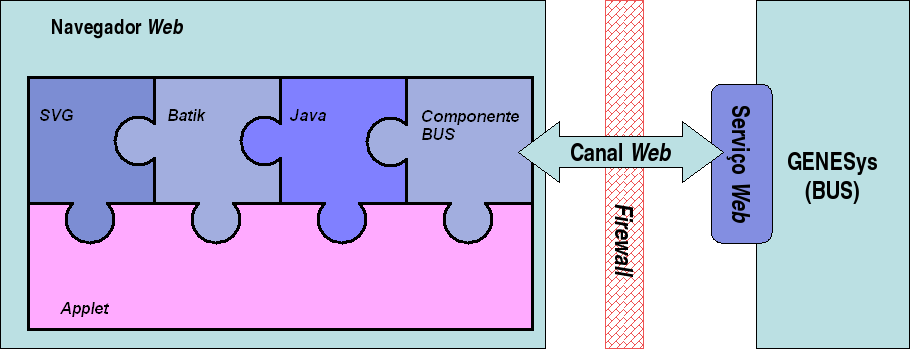
\includegraphics[width=0.86\textwidth]{puzzle}
    \caption{Arquitectura da Solução Proposta}
    \label{fig:arch}
  \end{center}
\end{figure}

Loren ipsum dolor sit amet, consectetuer adipiscing elit. 
Praesent sit amet sem. Maecenas eleifend facilisis leo. Vestibulum et
mi. Aliquam posuere, ante non tristique consectetuer, dui elit
scelerisque augue, eu vehicula nibh nisi ac est. Suspendisse elementum
sodales felis. Nullam laoreet fermentum urna. 

Duis eget diam. In est justo, tristique in, lacinia vel, feugiat eget,
quam. Pellentesque habitant morbi tristique senectus et netus et
malesuada fames ac turpis egestas. Fusce feugiat, elit ac placerat
fermentum, augue nisl ultricies eros, id fringilla enim sapien eu
felis. Vestibulum ante ipsum primis in faucibus orci luctus et
ultrices posuere cubilia Curae; Sed dolor mi, porttitor quis,
condimentum sed luctus. 

\subsection{Exemplo de Tabela}

É apresentado na Tabela~\ref{tab:exemplo1} um exemplo de tabela
flutuante e na Tabela~\ref{tab:exemplo2} um exemplo de tabela
flutuante, um pouco mais complicada.

\begin{table}[t]
  \centering
  \caption{Uma Tabela Simples}
\begin{tabular}{| l | p{45mm} |}
	\hline
\textbf{Acrónimo} & \textbf{Significado}\\
	\hline
	\hline
        ADT   & \emph{Abstract Data Type}\\\hline
        ANDF  & \emph{Architecture-Neutral Distribution Format}\\\hline
        API   & \emph{Application Programming Interface}\\
	\hline
\end{tabular}
  \label{tab:exemplo1}
\end{table}

Integer quis pede. Fusce nibh. Fusce nec erat vel mi condimentum
convallis. Sed at tortor non mauris pretium aliquet. In in lacus in
dolor molestie dapibus. Suspendisse potenti. Pellentesque sagittis
porta erat. Mauris sodales sapien id augue. Nam eu dolor. Donec sit
amet turpis non orci rhoncus commodo. Etiam condimentum commodo
libero.

Mauris pede. Curabitur faucibus dictum nibh. Proin tincidunt diam
vitae mauris. Sed hendrerit dolor vel ipsum. Nullam dapibus. Vivamus
tellus diam, egestas sit amet, vulputate non, vulputate id, eros. Nunc
sit amet nibh eget nibh imperdiet ornare. Cras vehicula mattis
ipsum. Sed diam arcu, semper at, gravida vitae, fermentum et,
nulla. Aenean massa orci, tristique nec, rutrum id, fringilla eget,
erat. Curabitur nulla ipsum, aliquam sed, rutrum vitae, semper quis,
ante. Fusce at nunc in dolor condimentum tempor. Duis sit amet massa. 

Curabitur convallis nulla quis risus. Nulla mollis porttitor
purus. Fusce ultricies odio at ligula pellentesque suscipit. Nulla
velit libero, blandit a, aliquet quis, hendrerit id, arcu. Phasellus
porttitor porttitor purus. Suspendisse velit tortor, fringilla sit
amet, commodo a, ultrices et, mi. Donec eu metus in erat ornare
adipiscing. Praesent varius mi ac nunc. Vestibulum leo lacus,
elementum in, vestibulum sit amet, hendrerit at, justo. Sed sit amet
neque. Donec libero risus, commodo sit amet, dignissim ut, tincidunt
a, eros. Ut non lacus quis tortor mattis ullamcorper. Vivamus
consequat augue vel erat. Sed tincidunt. Sed leo eros, ornare a,
pulvinar non, mattis quis, nibh. Aliquam faucibus mi ac nisi.

Pellentesque habitant morbi tristique senectus et netus et malesuada
fames ac turpis egestas. Duis aliquet, libero sit amet ornare viverra,
augue erat interdum dolor, vitae tincidunt lorem erat a lacus. Sed
lectus nisi, auctor in, hendrerit a, molestie vel, lectus. Cum sociis
natoque penatibus et magnis dis parturient montes, nascetur ridiculus
mus. Duis lacinia tempor dui. Vivamus rhoncus, tellus a viverra
dignissim, pede dui adipiscing odio, non faucibus metus mi gravida
eros. Nullam a tellus ut velit elementum tempus. Aenean rutrum
convallis tellus. Vestibulum nulla ante, dapibus ut, lobortis ut,
varius sed, nisl. Fusce lobortis. Sed ac lorem. Nulla tincidunt nulla
eget leo. Maecenas ac lectus eu neque ultrices pharetra. Curabitur a
risus nec arcu placerat tempor. Suspendisse magna nisl, viverra a,
adipiscing eget, ornare ultricies, ligula. Maecenas eu ligula vitae
eros convallis dignissim. 

\begin{table}[t]
  \centering
  \caption{Uma Tabela Mais Complicada}
\begin{tabular}{|c|r@{.}lr@{.}lr@{.}l||r|}
	\hline
\multicolumn{8}{|c|}
	{\rule[-3mm]{0mm}{8mm}Iteração $k$ de $f(x_n)$} \\
\textbf{\em k}
	& \multicolumn{2}{c}{$x_1^k$}
	& \multicolumn{2}{c}{$x_2^k$}
	& \multicolumn{2}{c||}{$x_3^k$}
	& comentários \\ \hline \hline
0   & -0&3                 & 0&6                 &  0&7   & - \\
1   &  0&47102965 & 0&04883157 & -0&53345964  & $\delta<\epsilon$ \\
2   &  0&49988691 & 0&00228830 & -0&52246185  & $\delta < \varepsilon$ \\
3   &  0&49999976 & 0&00005380 & -0&523656   &   $N$ \\
4   &  0&5                 & 0&00000307 & -0&52359743  & \\
\vdots	& \multicolumn{2}{c}{\vdots}
	& \multicolumn{2}{c}{$\ddots$}
	& \multicolumn{2}{c||}{\vdots}  & \\
7   &  0&5   & 0&0    & \textbf{-0}&\textbf{52359878}
		 & $\delta<10^{-8}$ \\ \hline
\end{tabular}
  \label{tab:exemplo2}
\end{table}

Loren ipsum dolor sit amet, consectetuer adipiscing elit. 
Praesent sit amet sem. Maecenas eleifend facilisis leo. Vestibulum et
mi. Aliquam posuere, ante non tristique consectetuer, dui elit
scelerisque augue, eu vehicula nibh nisi ac est. Suspendisse elementum
sodales felis. Nullam laoreet fermentum urna. 

Duis eget diam. In est justo, tristique in, lacinia vel, feugiat eget,
quam. Pellentesque habitant morbi tristique senectus et netus et
malesuada fames ac turpis egestas. Fusce feugiat, elit ac placerat
fermentum, augue nisl ultricies eros, id fringilla enim sapien eu
felis. Vestibulum ante ipsum primis in faucibus orci luctus et
ultrices posuere cubilia Curae; Sed dolor mi, porttitor quis,
condimentum sed luctus. 

\section{Secção Exemplo}

Loren ipsum dolor sit amet, consectetuer adipiscing elit. 
Praesent sit amet sem. Maecenas eleifend facilisis leo. Vestibulum et
mi. Aliquam posuere, ante non tristique consectetuer, dui elit
scelerisque augue, eu vehicula nibh nisi ac est. Suspendisse elementum
sodales felis. Nullam laoreet fermentum urna. 

Duis eget diam. In est justo, tristique in, lacinia vel, feugiat eget,
quam. Pellentesque habitant morbi tristique senectus et netus et
malesuada fames ac turpis egestas. Fusce feugiat, elit ac placerat
fermentum, augue nisl ultricies eros, id fringilla enim sapien eu
felis. Vestibulum ante ipsum primis in faucibus orci luctus et
ultrices posuere cubilia Curae; Sed dolor mi, porttitor quis,
condimentum sed luctus. 

\section{Resumo e Conclusões}

Resumir e apresentar as conclusões que se podem tirar no fim deste
capítulo.

\chapter{Datasets and Validation}\label{chap:validation}

\section*{}

\section{Datasets}\label{sec:datasets}

\section{Result Validation}\label{sec:validation}

\chapter{Work Plan} \label{chap:workplan}

\section*{}

This chapter describes the general work plan for the thesis, in terms of
activities and their respective timings. Furthermore, we will discuss the
datasets that will be used in the work, their characteristics and provenience.
Lastly, we will address the subject of work evaluation and validation,
explaining how it will be conducted, both during and at the end of the project.

\section{Planning}\label{sec:planning}

Aside the preparation phase (already completed), the time available for the
thesis will span from February to July, 2014, roughly totalling twenty weeks. It
is essential to define a top level schedule beforehand, to ensure that
sufficient time will be allotted for every phase of the project and that the
timings of those phases are feasible. As such, Figure \ref{fig:gantt} represents
the division of the six main phases of the project, during the available period
of twenty weeks. Although each phase comprises several smaller tasks, we believe
that such a small granularity planning is not needed in this phase and will be
defined during the work's execution, as needed. Each main phase of the project
is composed as follows:

\begin{figure}[!ht]
  \begin{center}

    \begin{ganttchart}[
      y unit title=0.6cm,
      y unit chart=0.7cm,
      x unit=0.8cm,
      vgrid,hgrid,
      title height=1,
      bar/.style={fill=gray!50},
      progress label text={},
      bar height=0.4]{12}

      % Time labels
      \gantttitle{2014}{12} \\
      \gantttitle{February}{2}
      \gantttitle{March}{2}
      \gantttitle{April}{2}
      \gantttitle{May}{2}
      \gantttitle{June}{2}
      \gantttitle{July}{2} \\

      % Tasks
      \ganttbar{Information system development}{2}{4} \\
      \ganttbar{Assembly pipeline development}{4}{5} \\
      \ganttbar{Web platform development}{5}{6} \\
      \ganttbar{Transcriptome assembly}{7}{9} \\
      \ganttbar{Transcriptome analysis}{8}{10} \\
      \ganttbar{Thesis writing}{9}{11}

    \end{ganttchart}
  \end{center}
  \caption{Work distribution planning}
  \label{fig:gantt}
\end{figure}

\begin{description}

  \item \textbf{Information system development}
  comprises the design and development of the data management component of the
  project and will take roughly six weeks. Despite not being the most critical
  component, making it the first in the development timeline facilitates later
  data intensive phases like the transcriptome assembly and, at the same time,
  allows extensive testing and performance evaluation through usage. A
  substantial time allotted for this phase will be spent tackling the
  performance aspects of implementing a system for such large quantities of
  data, both in terms of database size and response times.

  \item \textbf{Assembly pipeline development}
  consists of the construction of the tool pipeline responsible for assembling
  the transcriptomes. At first, several of the already mentioned tools will be
  studied and tested against small datasets, in an effort to ascertain which are
  best suited to our particular problem. As the tools are selected, the pipeline
  itself will take shape, integrating the tools in sequence. Any actual
  development effort in this phase will be in the form of simple data format
  conversion scripts, since we will use existing assembly tools. Because of
  this, the estimated duration of this phase is only one month or four weeks,
  despite its critical importance to the project.

  \item \textbf{Web platform development}
  will take four weeks and comprises the design and implementation of the
  system's web front-end. The web platform will integrate the information and
  assembly systems, providing a user friendly interface for genetic data
  storage, management and assembly. From a technical standpoint it's a fairly
  trivial system, which explains why only four weeks were reserved to this
  phase.

  \item \textbf{Transcriptome assembly}
  is the first phase after concluding the development of the main components of
  the system. In this phase the developed system will be used to produce the
  assembled transcriptome, employing the given production dataset. This phase
  will take about six weeks, despite no implementation work taking place (saving
  some small system tweaks). This is because genome and, in this case,
  transcriptome assembly are resource and time intensive processes that can
  take several days, making the extra time necessary for both new and repeat
  experiments.

  \item \textbf{Transcriptome analysis}
  will consist in the usage of several data mining tools in order to try to
  explain the already mentioned RNA transcription mechanisms. This phase is
  expected to last about six weeks. Although not as resource demanding as the
  transcriptome assembly phase, this will require choosing and testing a new
  set of tools and possibly integrate them with the developed system.

  \item \textbf{Thesis writing}
  is the last phase of the project, with an expected six weeks allocated time.
  These last six weeks refer to a period to collect and report the obtained
  results and to make the final reviews to the produced content. However, it is
  expected that the thesis report will be worked on continuously from the start 
  of the project, in parallel with the other project phases.

\end{description}

\section{Experimental Data}\label{sec:datasets}

During this project there will be essentially three types of datasets used: read
data, genome data and test data. Each type of dataset has its own nature, origin
and purpose. We will use real genetic data from a fly species called \fly{},
commonly known as fruit fly, which can be seen in Figure \ref{fig:fly}. It is
one of the most frequently used organisms to provide its genetic data for these
kind of studies and work.

\begin{figure}[!htb]
  \begin{center}
    \leavevmode
    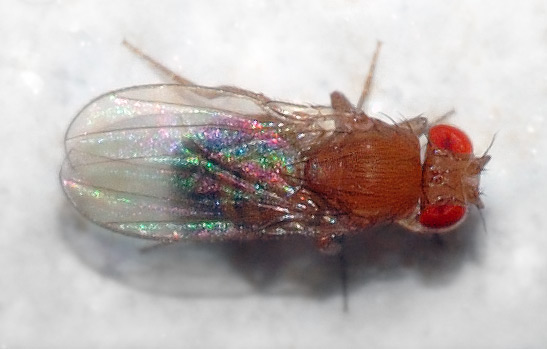
\includegraphics[width=0.6\textwidth]{d_melanogaster}
    \caption[Specimen of \fly, viewed from above]{Specimen of \fly, viewed from above\protect\footnotemark}
    \label{fig:fly}
  \end{center}
\end{figure}
\footnotetext{Image taken from \url{http://pt.wikipedia.org/wiki/Drosophila_melanogaster}.}

The read data will be made available during the project through IBMC. As stated,
this data consists of several short sequencing reads of the \fly{} genome. It is
this dataset that will be ultimately used for assembly and posterior data mining
analysis. It should be noted that this will be real data, experimentally
obtained in a laboratory for this project.

The genome data will consist of already assembled \fly{} genome(s), that will be
used as a reference in our own assembly process. This data will be obtained
through FlyBase\footnote{\url{www.flybase.org}}. FlyBase is an online and
publicly accessible database of \Fly{} genes and genomes. This database allows
its data to be downloaded in several formats, that can be either directly used
in our assembly pipeline, or be automatically converted by one of the created
conversion tools.

Lastly, we will use some small scale datasets for the test and calibration of the
assembly pipeline. Such datasets are usually shipped with the assembly tools
themselves. If needed, a combination of the two previous datasets can be used to
produce small scale test data for this purpose.

\section{Thesis Work Evaluation}\label{sec:eval}

In the second part of the project, that is the transcriptome assembly and
analysis phases, results evaluation and validation is essential. Even more so
when such results are typically evaluated from a molecular biology standpoint and
therefore are out of the scope of knowledge of the thesis itself. In such cases
we will have two evaluation methods at our disposal.

The first method is based on relevant metrics for the problems at hand, from
both the transcriptome assembly and data mining parts. Such metrics are usually
produced by the tools themselves. As for these metrics there is usually a well
defined range of expected results, which makes them a very important method of early
result evaluation, in the sense that they can be interpreted without a profound
knowledge about molecular biology.

The second method available is the evaluation by IMBC's technicians, that will
assist us whenever expert biology knowledge is required. This will ultimately be
the method that will provide a real measure of the success of the project.

Furthermore, IMBC's technicians will be essential during the entirety of the project. They
will help steer the project into its intended direction, giving some insight
about their expectations towards the system. Project phases like the
implementation of the information system or the transcriptome analysis will be
driven by their feedback, giving us a sense about what should be done. Lastly,
they will also be present throughout the project to help with any biology
related questions that arise.


%%----------------------------------------
%% Final materials
%%----------------------------------------

%% Bibliography
%% Comment the next command if BibTeX file not used
%% bibliography is in ``myrefs.bib''
\PrintBib{myrefs}

%% comment next 2 commands if numbered appendices are not used
%\appendix
%\chapter{Loren Ipsum} \label{ap1:loren}

Depois das conclusões e antes das referências bibliográficas,
apresenta-se neste anexo numerado o texto usado para preencher a
dissertação.

\section{O que é o \emph{Loren Ipsum}?}

\emph{\textbf{Lorem Ipsum}} is simply dummy text of the printing and
typesetting industry. Lorem Ipsum has been the industry's standard
dummy text ever since the 1500s, when an unknown printer took a galley
of type and scrambled it to make a type specimen book. It has survived
not only five centuries, but also the leap into electronic
typesetting, remaining essentially unchanged. It was popularised in
the 1960s with the release of Letraset sheets containing Lorem Ipsum
passages, and more recently with desktop publishing software like
Aldus PageMaker including versions of Lorem Ipsum~\citep{kn:Lip08}. 

\section{De onde Vem o Loren?}

Contrary to popular belief, Lorem Ipsum is not simply random text. It
has roots in a piece of classical Latin literature from 45 BC, making
it over 2000 years old. Richard McClintock, a Latin professor at
Hampden-Sydney College in Virginia, looked up one of the more obscure
Latin words, consectetur, from a Lorem Ipsum passage, and going
through the cites of the word in classical literature, discovered the
undoubtable source. Lorem Ipsum comes from sections 1.10.32 and
1.10.33 of ``de Finibus Bonorum et Malorum'' (The Extremes of Good and
Evil) by Cicero, written in 45 BC. This book is a treatise on the
theory of ethics, very popular during the Renaissance. The first line
of Lorem Ipsum, ``Lorem ipsum dolor sit amet\ldots'', comes from a line in
section 1.10.32.

The standard chunk of Lorem Ipsum used since the 1500s is reproduced
below for those interested. Sections 1.10.32 and 1.10.33 from ``de
Finibus Bonorum et Malorum'' by Cicero are also reproduced in their
exact original form, accompanied by English versions from the 1914
translation by H. Rackham.

\section{Porque se usa o Loren?}

It is a long established fact that a reader will be distracted by the
readable content of a page when looking at its layout. The point of
using Lorem Ipsum is that it has a more-or-less normal distribution of
letters, as opposed to using ``Content here, content here'', making it
look like readable English. Many desktop publishing packages and web
page editors now use Lorem Ipsum as their default model text, and a
search for ``lorem ipsum'' will uncover many web sites still in their
infancy. Various versions have evolved over the years, sometimes by
accident, sometimes on purpose (injected humour and the like). 

\section{Onde se Podem Encontrar Exemplos?}

There are many variations of passages of Lorem Ipsum available, but
the majority have suffered alteration in some form, by injected
humour, or randomised words which don't look even slightly
believable. If you are going to use a passage of Lorem Ipsum, you need
to be sure there isn't anything embarrassing hidden in the middle of
text. All the Lorem Ipsum generators on the Internet tend to repeat
predefined chunks as necessary, making this the first true generator
on the Internet. It uses a dictionary of over 200 Latin words,
combined with a handful of model sentence structures, to generate
Lorem Ipsum which looks reasonable. The generated Lorem Ipsum is
therefore always free from repetition, injected humour, or
non-characteristic words etc. 


%% Index
%% Uncomment next command if index is required
%% don't forget to run ``makeindex pdis-en'' command
%\PrintIndex

\end{document}
